%%%%%%%%%%%%%%%%%%%%%%%%%%%%%%%%%%%%%%%%%%%%%%%%%%%%%%%%%%%%%%%%%%%%%%%%%%%%%%%

\begin{frame}{}
	\begin{bibunit}[abbrv]
		\nocite{Holt1999b}
		\putbib
	\end{bibunit}
\end{frame}

%%%%%%%%%%%%%%%%%%%%%%%%%%%%%%%%%%%%%%%%%%%%%%%%%%%%%%%%%%%%%%%%%%%%%%%%%%%%%%%	
\begin{frame}[plain]
	\frametitle{Plant model without control}
		\begin{textblock*}{60mm}(65mm,25mm)
			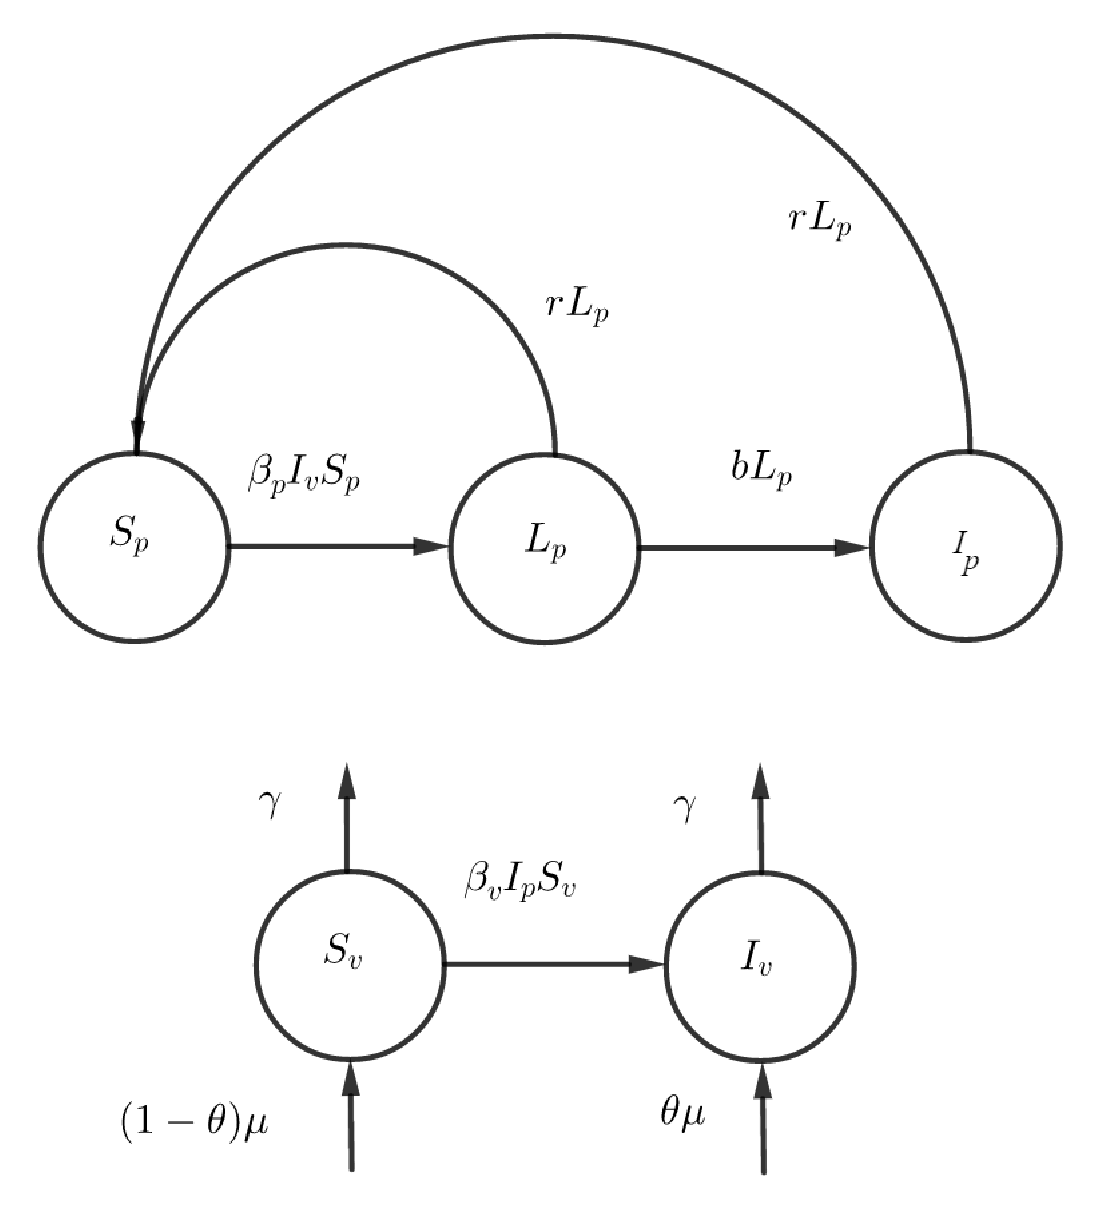
\includegraphics[width=\linewidth]{Feathergraphics/plant_diagram.eps}
		\end{textblock*}
		\begin{textblock*}{60mm}(2mm,25mm)
			\begin{graybox}{Hypothesis:}
				
				\begin{itemize}
					\item<1-> Plants become latent by infected vectors,
					\item<2-> replanting latent and infected plants,
					\item<3-> latent plants become infectious plants,
					\item<4-> vectors become infected by infected plants,
					\item<5-> vectors die or depart per day,
					\item<6-> immigration from alternative hosts.
				\end{itemize}
			\end{graybox}	
		\end{textblock*}
\end{frame}

%%%%%%%%%%%%%%%%%%%%%%%%%%%%%%%%%%%%%%%%%%%%%%%%%%%%%%%%%%%%%%%%%%%%%%%%%%%%%%%%
\subsection{Model without control}
	\begin{frame}[plain]
		\begin{textblock*}{61mm}(1mm,5mm)
			\begin{greenbox}{}
				\begin{align*}
				\frac{dS_p}{dt} &=
				-\beta_p S_p I_v +\textcolor{capri}{r}(L_p +  I_p),\\
				\frac{dL_p}{dt} &= 
				\beta_p S_p I_v -b L_p-\textcolor{capri}{r} L_p,\\
				\frac{dI_p}{dt} &=
			 b L_p - \textcolor{capri}{r} I_p,\\
				\frac{dS_v}{dt} &=
				-\beta_v S_v I_p - \textcolor{cadmiumorange}{\gamma} S_v   +(1-\theta)\mu,\\
				\frac{dI_v}{dt} &=
				\beta_v S_v I_p -\textcolor{cadmiumorange}{\gamma} I_v	+\theta\mu,\\
				S_p(0) &= S_{p_0}, L_p(0) = L_{p_0}, I_p(0) = I_{p_0},\\
				S_v(0) &= S_{v_0}, I_v(0) = I_{v_0}.
				\end{align*}
			\end{greenbox}
		\end{textblock*}
		\only<2>{
			\begin{textblock*}{50mm}(65mm,5mm)
				\begin{tabular}{|c |c |l |} 
					\hline
					Par. & Unit & value \\ [0.5ex] 
					\hline
					$\beta_p$ & vector$^{-1}$day$^{-1}$ & 0.1\\ 
					\hline
					$r$ & day$^{-1}$ & 0.01 \\
					\hline
					$b$ & day$^{-1}$ & 0.075\\
					\hline
					$\gamma$ & day$^{-1}$ & 0.06\\
					\hline
					$\mu$ & plant$^{-1}$day$^{-1}$ & 0.3\\
					\hline
					$\theta$ & proportion & 0.2\\
					\hline
					$\beta_v$ & plant$^{-1}$day$^{-1}$ & 0.003\\ 
					\hline
				\end{tabular}
			\end{textblock*}
		}
		\only<1>{
			\begin{textblock*}{60mm}(65mm,5mm)
				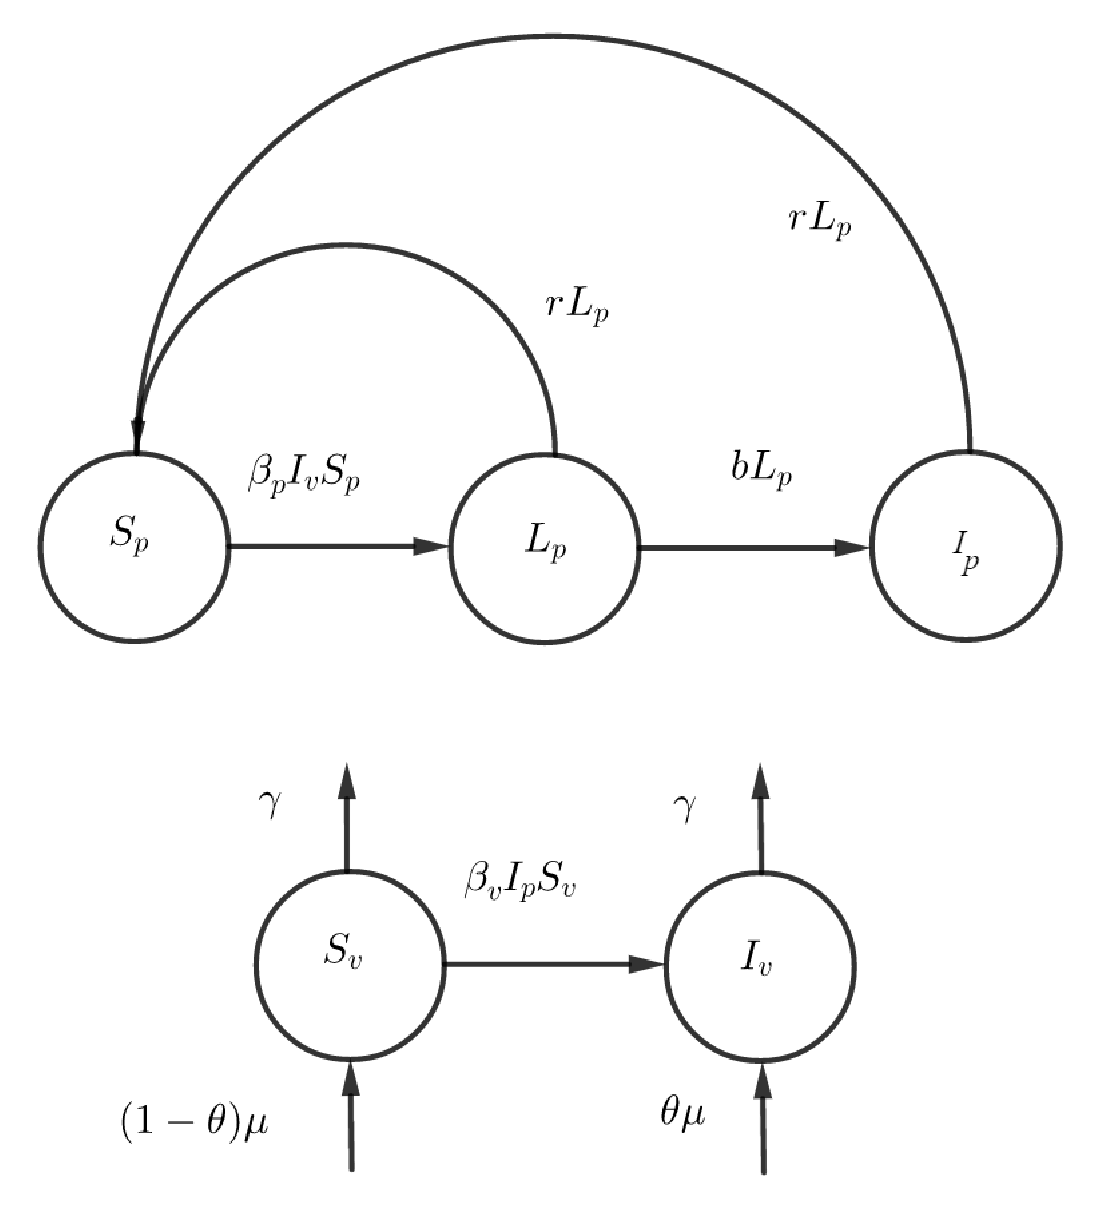
\includegraphics[width=\linewidth]{Feathergraphics/plant_diagram.eps}
			\end{textblock*}
		}
		\only<3>
		{
			\begin{textblock*}{55mm}(70mm,20mm)
				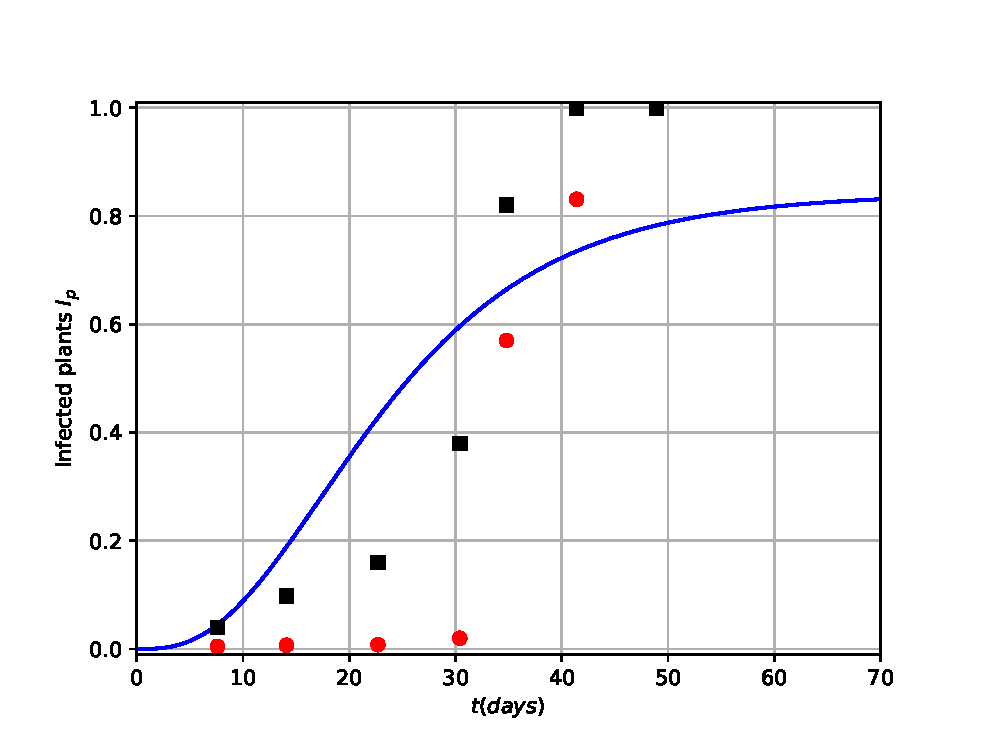
\includegraphics[width=\linewidth]{Feathergraphics/Simulation_data.eps}
			\end{textblock*}
		}
	\end{frame}
%%%%%%%%%%%%%%%%%%%%%%%%%%%%%%%%%%%%%%%%%%%%%%%%%%%%%%%%%%%%%%%%%%%%%%%%%%%%%%%%
	\begin{frame}[plain]
	
			\begin{textblock*}{55mm}(5mm,18mm)	
				\only<1,2,3>
				{
				\begin{greenbox}{Basic reproductive number:}
					\begin{equation*}
					R_0=\sqrt{\frac{\beta_v\mu b\beta_p}{r^2(r+b)\gamma}}.
					\end{equation*}
				\end{greenbox}
				}
			\only<2>
			{	
				\begin{textblock*}{70mm}(5mm,45mm)
					\begin{yellowbox}{}
					
						If $R_0<1,$
						\begin{equation*}
						\lim\limits_{t\rightarrow \infty}(S_p,L_p,I_p,S_v,I_v)=(N_p,0,0,\frac{\mu}{\gamma},0).
						\end{equation*}
					\end{yellowbox}
				\end{textblock*}
			}
				\only<3>
				{
				\begin{textblock*}{70mm}(5mm,45mm)
					\begin{yellowbox}{}
					If $R_0>1,$
						\begin{equation*}
							\lim\limits_{t\rightarrow \infty}(S_p,L_p,I_p,S_v,I_v)=(S_p^*,L_p^*,I_p^*,S_v^*,I_v^*).
						\end{equation*}
				
					\end{yellowbox}
				\end{textblock*}
				}
			
		\end{textblock*}
		\begin{textblock*}{50mm}(77mm,35mm)
			\only<2>
			{
				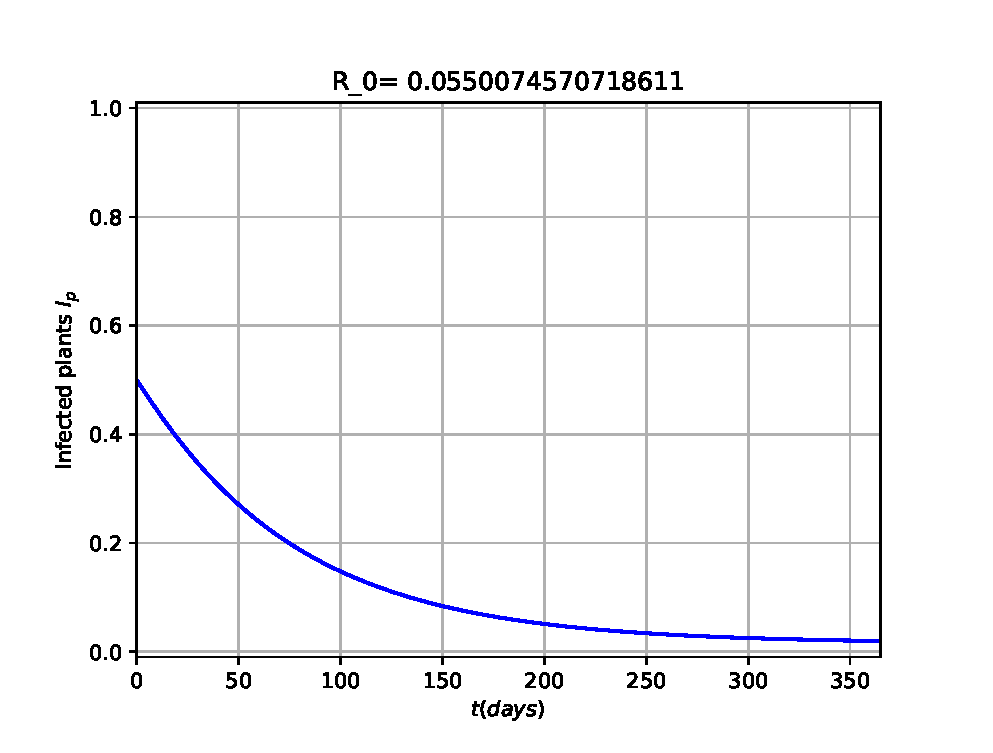
\includegraphics[width=\linewidth]{Feathergraphics/Tomato_simulation_1.eps}
			}
			\only<3>
			{
				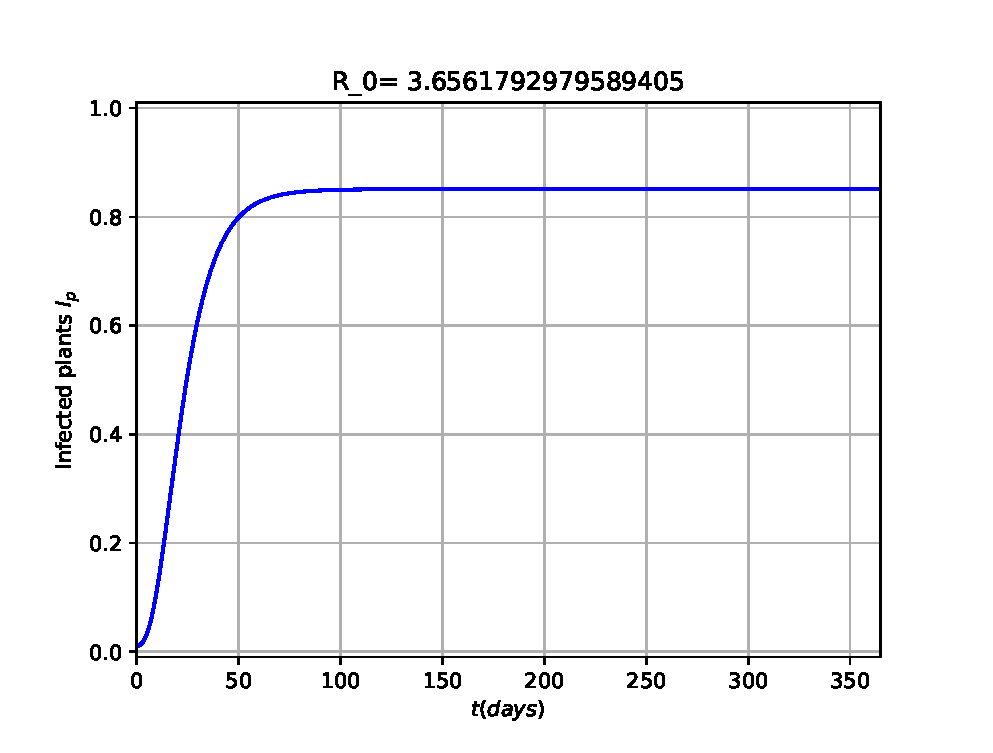
\includegraphics[width=\linewidth]{Feathergraphics/Tomato_simulation_2.eps}
			}
		\end{textblock*}	
	\end{frame}
%%%%%%%%%%%%%%%%%%%%%%%%%%%%%%%%%%%%%%%%%%%%%%%%%%%%%%%%%%%%%%%%%%%%%%%%%%%%%%%%
\subsection{Controlled Model}

	\begin{frame}[plain]\frametitle{Controlled model}
		\only<1,2>
		{
			\begin{textblock*}{70mm}(1mm,10mm)
			\begin{greenbox}{}
				\begin{align*}
				\frac{dS_p}{dt} &=
				-\beta_p S_p I_v +\textcolor{capri}{r}(L_p +  I_p),\\
				\frac{dL_p}{dt} &= 
				\beta_p S_p I_v -b L_p-\textcolor{capri}{r} L_p,\\
				\frac{dI_p}{dt} &=
				b L_p - \textcolor{capri}{r} I_p,\\
				\frac{dS_v}{dt} &=
				-\beta_v S_v I_p - \textcolor{cadmiumorange}{\gamma} S_v   +(1-\theta)\mu,\\
				\frac{dI_v}{dt} &=
				\beta_v S_v I_p -\textcolor{cadmiumorange}{\gamma} I_v	+\theta\mu,\\
				S_p(0) &= S_{p_0}, L_p(0) = L_{p_0}, I_p(0) = I_{p_0},\\
				S_v(0) &= S_{v_0}, I_v(0) = I_{v_0}.
				\end{align*}
			\end{greenbox}
		\end{textblock*}
		
		}
		\only<3,4>
		{
			\begin{textblock*}{70mm}(1mm,10mm)
				\begin{greenbox}{}
					\begin{align*}
						\frac{dS_p}{dt} &=
						-\beta_p S_p I_v +(\textcolor{capri}{r +u_1})L_p + (\textcolor{capri}{r + u_2}) I_p,\\
						\frac{dL_p}{dt} &=
						\beta_p S_p I_v -b L_p -(\textcolor{capri}{r + u_1})L_p,\\
						\frac{dI_p}{dt} &= 
						b L_p - (\textcolor{capri}{r + u_2}) I_p,\\
						\frac{dS_v}{dt} &=
						-\beta_v S_v I_p - (\textcolor{cadmiumorange}{\gamma+u_3}) S_v +(1-\theta)\mu,\\
						\frac{dI_v}{dt} &=
						\beta_v S_v I_p -(\textcolor{cadmiumorange}{\gamma+u_3}) I_v +\theta\mu,				
					\end{align*}
				\end{greenbox}
			\end{textblock*}
		}
		\only<2,3,4>
		{
			\begin{textblock*}{53mm}(73mm,10mm)
				\begin{yellowbox}{Controls:}
					\begin{itemize}
						\item $u_1$: replanting latent plant,
						\item $u_2$: replanting infected plants,
						\item $u_3$: fumigation,
					\end{itemize}
					\tcblower
						$$u^{min}_i<u_i<u^{max}_i.$$
				\end{yellowbox}
			\end{textblock*}
		}
		\only<4>
		{
			\begin{textblock*}{115mm}(8mm,65mm)
				\begin{yellowbox}{Cost Functional}
					\begin{align*}
					\int_{0}^T	(A_1 I_p(t) + A_2 L_p(t) + A_3 I_v(t) + c_1 u_1(t)^2 + c_2 u_2(t)^2 + c_3 u_3(t)^2) dt,
					\end{align*}
				\end{yellowbox}
			\end{textblock*}
		}
		\end{frame}
%%%%%%%%%%%%%%%%%%%%%%%%%%%%%%%%%%%%%%%%%%%%%%%%%%%%%%%%%%%%%%%%%%%%%%%%%%%%%%%%
	\begin{frame}[plain]
		\begin{textblock*}{120mm}(2mm,2mm)
			\begin{yellowbox}{OC}
				\begin{align*}
				\min_{\bar{u}(\cdot)\in \mathcal{U}_{x_0}[t_0,T]}J(u_1,u_2,u_3)
				\end{align*}
				s.t.
				\begin{equation*}
					%\left\{ 
					\begin{aligned}
						\frac{dS_p}{dt} &=
						 -\beta_p S_p I_v +(r +u_1)L_p + (r + u_2) I_p,
						 \\
						\frac{dL_p}{dt} &=
						\beta_p S_p I_v -b L_p -(r + u_1)L_p,
						\\
						\frac{dI_p}{dt} &= 
						b L_p - (r + u_2) I_p,
						\\
						\frac{dS_v}{dt} &=
						-\beta_v S_v I_p - (\gamma+u_3) S_v +(1-\theta)\mu,
						\\
						\frac{dI_v}{dt} &=
						\beta_v S_v I_p -(\gamma+u_3) I_v +\theta\mu,
						\\
						&S_p(0) = S_{p_0}, L_p(0) = L_{p_0},
						\\
						&I_p(0) = I_{p_0},S_v(0) = S_{v_0}, I_v(0) = I_{v_0}.
						\\
						&u_i(t)\in[0,u_i^{max}]
						\end{aligned}%\right.
				\end{equation*}
			\end{yellowbox}
		\end{textblock*}
	\end{frame}
%%%%%%%%%%%%%%%%%%%%%%%%%%%%%%%%%%%%%%%%%%%%%%%%%%%%%%%%%%%%%%%%%%%%%%%%%%%%%%%%
